\documentclass[12pt,a4paper]{article}
\usepackage{amsmath,amsthm,amssymb,graphicx,hyperref,float,mathalpha}
\usepackage[left=1.2in,right=1in,top=1in,bottom=1in]{geometry}
\usepackage[english]{babel}
\usepackage{xcolor}
\usepackage{textcomp}
\usepackage[normalem]{ulem}
\usepackage[T1]{fontenc}
\useunder{\uline}{\ul}{}
\usepackage{listings}
\usepackage{color}
\usepackage{graphicx} % Required for inserting images
\usepackage{listings}
\usepackage{fancyvrb}
\definecolor{mygreen}{rgb}{0,0.6,0}
\definecolor{mygray}{rgb}{0.5,0.5,0.5}
\definecolor{mymauve}{rgb}{0.58,0,0.82}
\definecolor{backcolour}{rgb}{0.95,0.95,0.92}
\usepackage{booktabs}
\lstset{ %
  backgroundcolor=\color{backcolour},   % choose the background color
  numberstyle=\tiny,
  basicstyle=\footnotesize,        % size of fonts used for the code
  breaklines=true,                 % automatic line breaking only at whitespace
  captionpos=b,                    % sets the caption-position to bottom
  commentstyle=\color{mygreen},    % comment style
  escapeinside={\%*}{*)},          % if you want to add LaTeX within your code
  keywordstyle=\color{blue},       % keyword style
  stringstyle=\color{mymauve},     % string literal style
  numbers=left,                    
  numbersep=5pt
}
\usepackage{comment}
\newcommand\tab[1][5mm]{\hspace*{#1}}
\newcommand\taba[1][10mm]{\hspace*{#1}}
\newtheorem{thm}{Teorema}[section]
\newtheorem{lem}[thm]{Lema}
\newtheorem{cor}[thm]{Corolarul}
\newtheorem{prop}[thm]{Propozi\c tia}
\theoremstyle{definition}
\newtheorem{defn}{Defini\c tia}[section]
\theoremstyle{remark}
\newtheorem{rem}{Remarca}[section]
\newtheorem{exmp}{Exemplul}[section]
\begin{document}
\thispagestyle{empty}
\begin{center}
\begin{figure}[h!]
\vspace{-20pt}
\begin{center}

\includegraphics[width=100pt]{FMI-03.png}
\end{center}
\end{figure}

{\large{\bf UNIVERSITATEA DE VEST DIN TIMI\c SOARA

FACULTATEA DE MATEMATIC\u A \c SI INFORMATIC\u A}}

\vspace{100pt}
{\huge {\bf Verificarea Re\c telelor Neuronale folosind Alpha-Beta CROWN \c si NeuralSAT pentru Benchmark-ul Acas XU}}

\vspace{100pt}
\end{center}
\vspace{175pt}
\noindent Bordea Liviu Valentin\\
\noindent Ciurdea Roberta Carla\\
\noindent Burcea Adina M\u ad\u alina \hfill Conf. Dr. M\u ad\u alina Era\c scu\\


\newpage
\normalsize{}
\begin{center}
        \textbf{\selectfont\section* {Abstract}}
            \end{center}
        \vspace{0.7cm}
        \par
Neural networks are being applied to a growing variety of applications, including safetycritical domains like autonomous vehicles and aircraft, due to their ability to approximate complex functions from limited datasets and adapt by continuing to learn from real-world data after deployment.\par
This report is focused on the installation of the two tools: alpha-beta-CROWN and NeuralSAT, which are applied to the Acas XU benchmark. \par
The structure of the report is based on 4 chapters. The first chapter presents the description of the chosen data set, Acas XU, the next one includes the installation of the 2 tools: alpha-beta-CROWN, NeuralSAT, and the last 2 chapters present the running of alpha-beta-CROWN, NeuralSAT on Acas XU and the final conclusions together with the problems encountered on the entire configuration of the chosen dataset.



\newpage
\section{Introducere}
Verificarea DNN (Deep Neural Network) este un proces de confirmare a faptului că, pentru fiecare posibilă intrare, ieșirea rețelei neurale satisface proprietățile dorite. Cu alte cuvinte, este vorba despre verificarea relațiilor dintre intrarea și ieșirea rețelei neurale pentru a vedea dacă proprietățile specifice dintre ele sunt respectate.\par
VNN-COMP reprezintă Competiția de Verificare a Rețelelor Neurale, care s-a desfășurat anual timp de trei ani și a avut numeroși cercetători activi în acest domeniu ca participanți.\par
Din cea mai recentă ediție a VNN-COMP, am selectat doua instrumente care au obținut cele mai bune performanțe, au participat la cele mai multe benchmark-uri si au furnizat documentație suficientă pentru raportul nostru. Ca si benchmark, am ales AcasXU deoarece este unul dintre cele mai complexe dataset-urile, considerandu-l cel mai potrivit pentru acest proiect.\par
Într-un sistem critic pentru securitate precum ACAS Xu, un atacator poate exploata cu ușurință o situație limită gestionată incorect pentru a cauza daune semnificative, punând în pericol mii de vieți. Metodele existente pentru testarea rețelelor neurale în fața situațiilor limită se concentrează pe identificarea exemplelor adversare \cite{reluplex}. \par
\section{Descrierea Dataset-ului}
{\bf ACAS XU\cite{introduction} (Automated Collision Avoidance System)} este un sistem de evitare a coliziunilor aer-la-aer proiectat pentru aeronave fără pilot, care emite sfaturi privind virajele orizontale pentru a evita o aeronavă intruză. Datorită utilizării unei tabele de căutare mari în proiectare, s-a propus o comprimare a politicii cu ajutorul unei rețele neurale. \par
{\bf Funcționalitatea Rețelei}. Sistemul ACAS Xu mapează variabilele de intrare la recomandările de acțiune. Fiecare recomandare este asignată un scor, cu cel mai mic scor corespunzător celei mai bune acțiuni. Starea de intrare este compusă din șapte dimensiuni (prezentate în Figure 1) care reprezintă informațiile determinate din măsurătorile senzorilor: \par
(i) $\rho$: Distanța de la propria navă la intrus. \par
(ii) $\theta$ : Unghiul față de intrus în raport cu direcția de îndreptare a propriei nave. \par
(iii) $\psi$: Unghiul de îndreptare al intrusului în raport cu direcția de îndreptare a propriei nave. \par
(iv) vown: Viteza propriei nave. \par
(v) vint: Viteza intrusului. \par

\begin{figure}[h!]
  \centering
    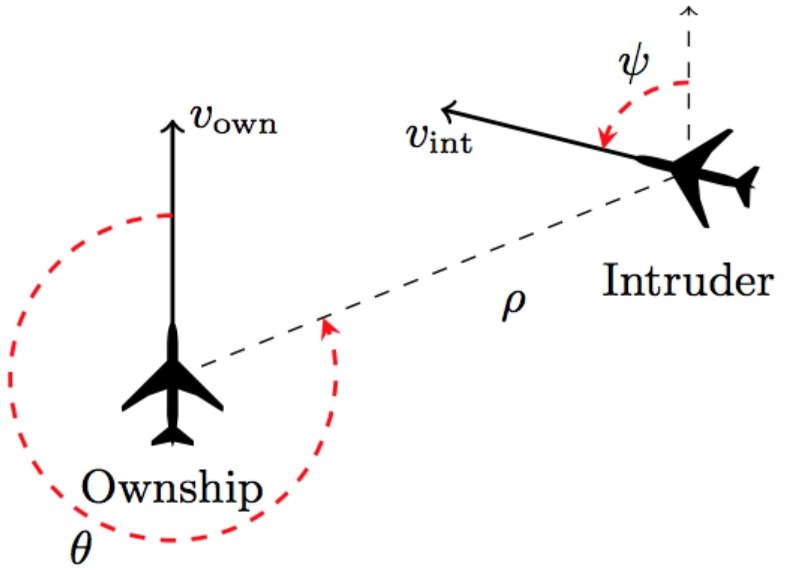
\includegraphics[width=0.6\textwidth]{ACASXU.jpg}
    \caption{Sistemul ACAS Xu (adaptat din (Katz et al. 2017)) \cite{abstraction_art}}
\end{figure}
Există cinci ieșiri care reprezintă diferitele recomandări orizontale pe care le poate primi propria navă: Fără Conflict (COC), dreapta slabă, dreapta puternică, stânga slabă sau stânga puternică. Slab și puternic înseamnă rate de îndreptare de 1.5 $^{\circ}$ /s și 3.0 $^{\circ}$ /s, respectiv. \par

Sistemul de evitare a coliziunilor cu aeronave fără pilot X (ACAS Xu) foloseste rețele neuronale pentru a anticipa cele mai bune acțiuni optime în funcție de locația și viteza avioanelor atacatoare din apropiere. A fost testat cu succes de NASA și FAA și este în program pentru a fi instalat la peste 30.000 de aeronave de pasageri și cargo la nivel mondial, precum și în flotele Marinei SUA. \cite{initial_separation}\par
{\bf Utilitate.} Dosarul de unde se poate găsi benchmark-ul ACAS Xu, conține fișierele .onnx și .vnnlib utilizate pentru această categorie, și poate fi descarcat de \href{https://github.com/ChristopherBrix/vnncomp2023_benchmarks/tree/main/benchmarks/acasxu}{aici}.  \par
Fișierul \texttt{acasxu\_instances.csv} conține lista completă a instanțelor de benchmark, câte una pe linie: \texttt{onnx\_file}, \texttt{vnn\_lib\_file},  \texttt{timeout\_secs}. Fișierele .vnnlib și .csv au fost create cu ajutorul scriptului generate.py inclus. Fișierul cu extensia ".onnx" reprezintă modelul neuronal, iar cel cu extensia ".vnnlib" specificațiile. \par
{\bf Rețele (onnx):} ACASXu consta în zece proprietăți definite pentru 45 de rețele neurale utilizate pentru a emite avertismente de viraj aeronautic pentru evitarea coliziunilor. Rețelele neurale au 300 de neuroni aranjați în 6 straturi, cu funcții de activare ReLU. Există cinci intrări corespunzătoare stării aeronavelor și cinci ieșiri ale rețelei, unde ieșirea minimă este utilizată ca avertisment de viraj produs în cele din urmă de sistem.\par
{\bf Specificatii (vnnlib):} Sunt utilizate cele zece proprietăți originale (vnnlib), unde proprietățile 1-4 sunt verificate pe toate cele 45 de rețele, așa cum s-a făcut ulterior de catre autorii originali. Proprietățile 5-10 sunt verificate pe o singură rețea. Prin urmare, numărul total de benchmark-uri este de 186.\par
Ca standard pentru VNN-COMP 2022, instrumentele sunt compatibile cu modelele de rețele neurale în formatul Open Neural Network Exchange (ONNX), care pot fi convertite ușor din alte formate de fișiere ale altor cadre de învățare automată. Pentru specificații, se utilizează formatul VNNLIB, creat în mod specific pentru competiție. Acest format de specificații constă în declarații de variabile și afirmații (assertion statements), așa cum este prezentat in Figure 2.\par
\begin{figure}[h!]
  \centering
    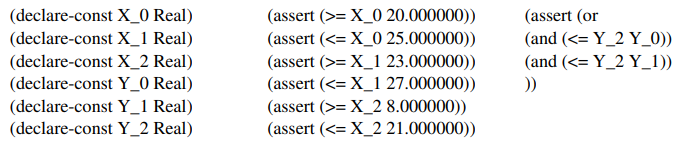
\includegraphics[width=.8\textwidth]{standard.png}
    \caption{Formatul Standard al Fișierelor VNNLIB}
    \cite{format}
\end{figure}


\section{Instalarea tool-urilor}
\subsection{Alpha Beta-CROWN}
Alpha-beta-CROWN\cite{abcrown} este un verificator de rețele neurale bazat pe un cadru eficient de propagare a limitelor liniare și pe tehnica de branch and bound. Poate fi accelerat eficient pe unități de procesare grafică (GPU) și poate scala către rețele convoluționale relativ mari. \par
Pentru a instala Alpha Beta-CROWN, am folosit miniconda3 si sistemul de operare Linux Kali. \par
Dupa instalarea miniconda \cite{miniconda} și restartarea terminalului, a fost nevoie de clonarea folderului "alpha-beta-CROWN"\cite{git1} (Figure 3) și "auto\_LIRPA"\cite{git2} (Figure 4) de pe github folosind instrucțiunile: \par
\begin{lstlisting}[style=bashstyle]
    git clone --recursive https://github.com/Verified-Intelligence/alpha-beta-CROWN.git
    git clone https://github.com/Verified-Intelligence/auto_LiRPA
\end{lstlisting}


   
\begin{figure}[h!]
  \centering
    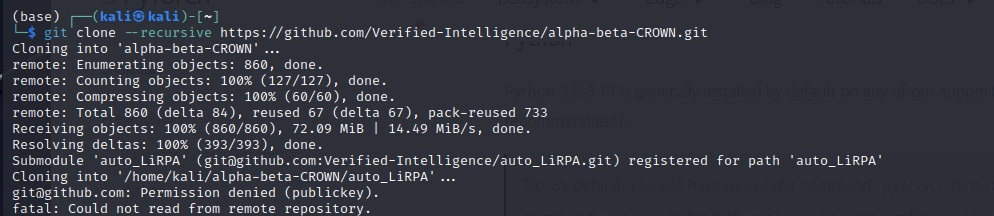
\includegraphics[width=1\textwidth]{a_b_crown.jpg}
    \caption{Clonarea Alpha-beta CROWN}
\end{figure}
\begin{figure}[h!]
  \centering
    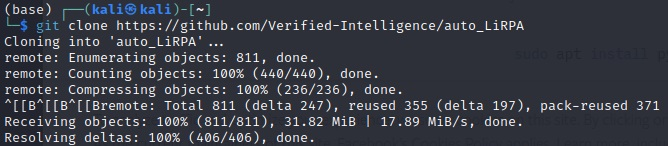
\includegraphics[width=0.8\textwidth]{libra.jpg}
    \caption{Clonarea Auto Lirpa}
\end{figure}

Am creat environmentul (Figure 6), și am activat alpha-beta-crown (Figure 5) folosind instrucțiunile: \par

\begin{lstlisting}[style=bashstyle]
    conda env create -f complete\_verifier/environment.yaml --name alpha beta-crown
    conda activate alpha-beta-crown
\end{lstlisting}
\begin{figure}[h!]
  \centering
    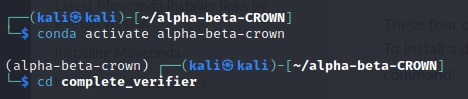
\includegraphics[width=0.5\textwidth]{linux2.jpg}
    \caption{Activarea tool-ului}
\end{figure}
\begin{figure}[h!]
  \centering
    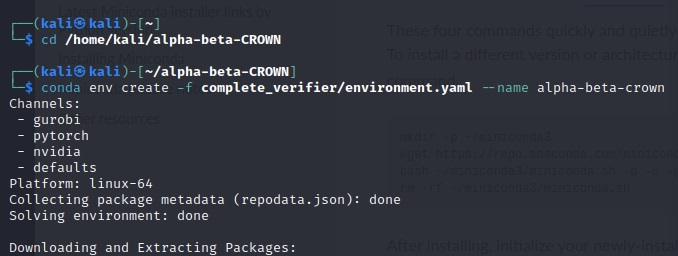
\includegraphics[width=0.6\textwidth]{kali.jpg}
    \caption{Crearea environmentului}
\end{figure}

Dupa activarea "alpha-beta-CROWN", a fost nevoie de instalarea unor pachete pentru a putea rula benchmark-ul. Aceste pachete sunt: onnx2pytorch, onnxruntime, onnxoptimizer, skl2onnx, torch, torchvision, pe care le-am instalat folosind urmatoarele instrucțiuni:\par
\begin{lstlisting}[style=bashstyle]
    pip install git+https://github.com/KaidiXu/onnx2pytorch.git  
    pip install onnxruntime==1.16.3
    pip install onnxoptimizer==0.3.13
    pip install skl2onnx==1.15.0
    pip install torchvision==0.15.1
    pip install torch==1.13.0 
\end{lstlisting}


\subsection{NeuralSAT}
NeuralSAT\cite{neuralsat} este o unealtă de verificare a rețelelor neurale profunde (DNN - Deep Neural Network). Integrează abordarea DPLL(T)\cite{dpllt} folosită în mod obișnuit în rezolvarea SMT cu un solver de teorie specializat pentru raționamentul DNN. NeuralSAT valorifică unitățile de procesare multistrat (multicores) și unitatea de procesare grafică (GPU) pentru eficiență și poate scala pentru rețele cu milioane de parametri. \par
Pentru a instala NeuralSAT, am folosit miniconda3 și sistemul de operare Linux Kali. \par
Dupa instalarea miniconda și restartarea terminalului, a fost nevoie de clonarea folderului "neuralsat"\cite{git3} (Figure 7) de pe github folosind instrucțiunea: \par
\begin{lstlisting}[style=bashstyle]
    git clone --recursive https://github.com/dynaroars/neuralsat.git
\end{lstlisting} \par
\begin{figure}[h!]
  \centering
    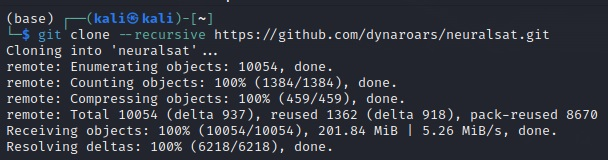
\includegraphics[width=0.7\textwidth]{neuralsat.jpg}
    \caption{Clonarea NeuralSAT}
\end{figure}
Am creat environmentul (Figure 8), și am activat neuralsat (Figure 9) folosind instrucțiunile: \par
\begin{lstlisting}[style=bashstyle]
    conda env create -f env.yaml
    conda activate neuralsat
\end{lstlisting}
\begin{figure}[!htb]
   \begin{minipage}{0.48\textwidth}
     \centering
     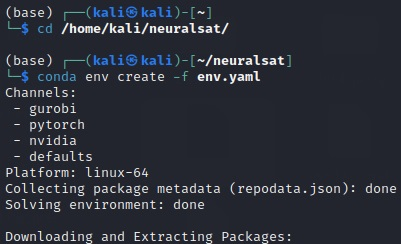
\includegraphics[width=.95\linewidth]{neuralsat_env.jpg}
     \caption{Crearea environmentului}\label{Fig:Data1}
   \end{minipage}\hfill
   \begin{minipage}{0.48\textwidth}
     \centering
     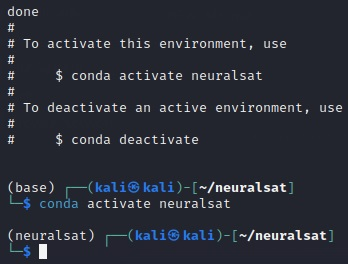
\includegraphics[width=.9\linewidth]{neuralsat_activate.jpg}
     \caption{Activarea tool-ului}\label{Fig:Data2}
   \end{minipage}
\end{figure}

\section{Rularea tool-urilor pentru dataset-ul ales}
Pentru a rula AcasXu, am descărcat arhiva care conține toate benchmark-urile din 2023 \cite{git4}. După descărcare, am dezarhivat folderul "acasxu" și componentele acestuia. Am creat un nou folder cu denumirea "vnncomp2023\_benchmarks" în care am creat folderul "benchmarks", unde am adaugat folderul "acasxu" dezarhivat și descărcat de pe github.  \par
Din cauza unor erori, a fost necesară adăugarea unei instrucțiuni în fișierul de configurare al benchmark-ului. Instrucțiunea este "device: cpu", astfel încat pytorch să utilizeze CPU în loc de GPU. \par

\subsection{Tool 1: Alpha-Beta CROWN}
Pentru a aplica benchmark-ul și a primi rezultatele am folosit urmatoarea instrucțiune pe care am rulat-o în folderul "complete\_verifier" aflat în "alpha-beta-CROWN": 
\begin{lstlisting}[style=bashstyle]
    python abcrown.py --config exp\_configs/vnncomp23/acasxu.yaml
\end{lstlisting}
Ca și rezultate, acestea pot fi vizualizate în fișierul  "rezultat\_abcrown.txt" \cite{ref1}, dar și in tabelul "results\_ABCROWN.csv"\cite{ref2} unde se pot observa diferențele dintre rezultatele de la competiția din 2023 și rezultatele la care am reusit să ajungem noi. Sumarul rezultatului se poate observa în Figure 10, iar în Figure 11 am evidențiat 3 tipuri de rezultate din fișierul "results\_ABCROWN.csv".\par
\begin{figure}[h!]
  \centering
    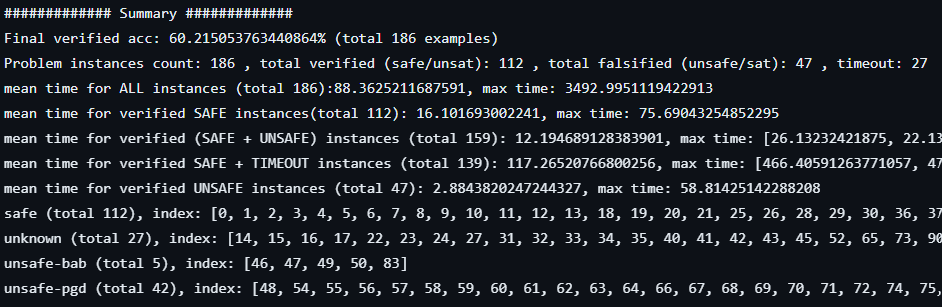
\includegraphics[width=0.8\textwidth]{rezultat.png}
    \caption{Sumar al rezultatului}
\end{figure}
\begin{figure}[h!]
  \centering
    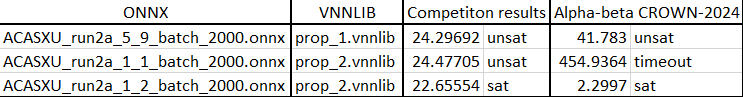
\includegraphics[width=0.9\textwidth]{csv.png}
    \caption{Exemple din fișierul results\_ABCROWN.csv}
\end{figure}

Programul a returnat un total de 47 de cazuri satifiabile (un-safe), 112 nesatisfiabile (safe) dar și 27 unknown (timeout). Figure 12 reprezintă procentul pe care fiecare tip de rezultat il reprezintă din totalul de 186 de instanțe. \par

\begin{figure}[!htb]
   \begin{minipage}{0.48\textwidth}
     \centering
     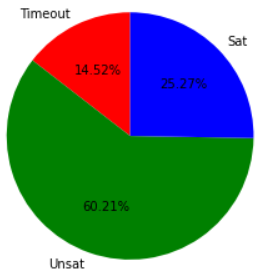
\includegraphics[width=.65\linewidth]{diag1.png}
     \caption{Diagrama Rezultatelor}\label{Fig:Data1}
   \end{minipage}\hfill
   \begin{minipage}{0.48\textwidth}
     \centering
     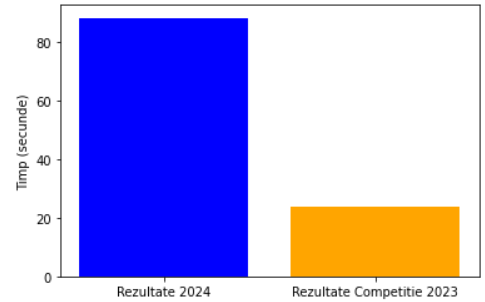
\includegraphics[width=1\linewidth]{diag2.png}
     \caption{Comparare Timp Mediu}\label{Fig:Data2}
   \end{minipage}
\end{figure}
Satifiabilitatea a fost aceeași ca și în rezultatele din 2023 pentru rezultatele care au fost verificate cu succes (sat, unsat), numai timpul de verificare a fost diferit într-o mare măsură. Timpul de verificare pentru rezultatele satifiabile a fost considerabil de mic față de cele nesatifiabile, deși în competiția trecută, timpii au fost asemanatori. De asemenea, timpul mediu de verificare pe care am reușit sa il obținem este cu aproximativ 269.86\% mai mare decat cel obținut în competiția din 2023 (Figure 13). Programul a afișat 27 de rezultate cu raspunsul "timeout" deoarece nu a reușit să ajungă la un rezultat, iar timpul de verificare a expirat. Am dedus că motivul pentru care timpul de verificare este considerabil mai mare și au fost mai multe rezultate de tipul "timeout" comparativ cu 2023, este incapabilitatea dispozitivului de pe care am rulat instrucțiunile (memorie insuficientă etc). \par
Ca și probleme întampinate în rularea dataset-ului cu tool-ul alpha-beta-crown au fost două situații în care în timpul rulării, programul s-a oprit cu secvența "killed" la diferite iterații probabil din cauza memoriei insuficiente (Figure 14). O alta problemă și cea mai neasteptată a fost atunci cand dispozitivul s-a închis brusc și a afișat instrucțiuni de recuperare (Figure 15).\par
\begin{figure}[!htb]
   \begin{minipage}{0.55\textwidth}
     \centering
     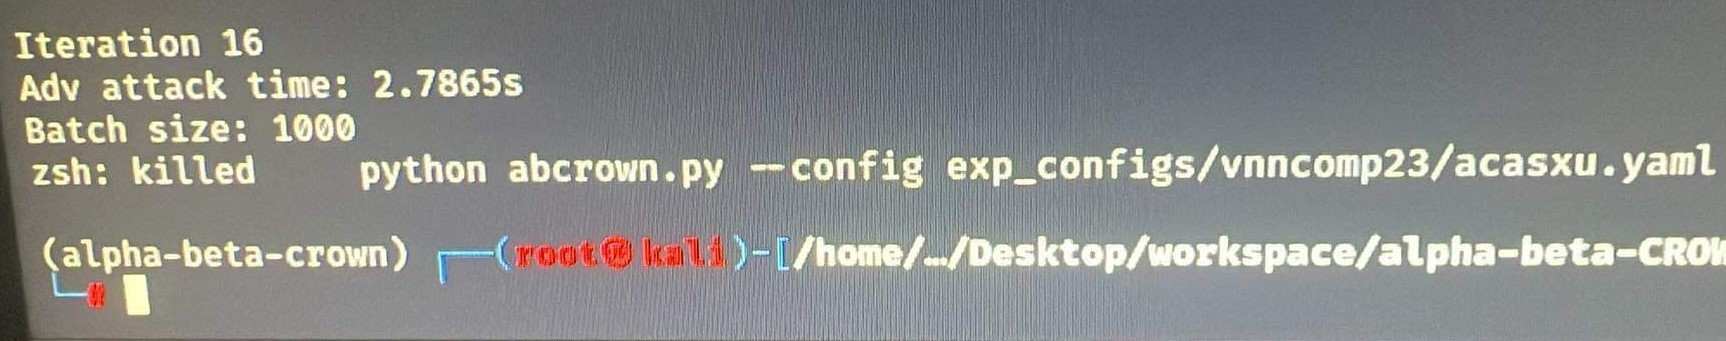
\includegraphics[width=.8\linewidth]{prob1.jpg}
     \caption{"Killed"}\label{Fig:Data1}
   \end{minipage}\hfill
   \begin{minipage}{0.48\textwidth}
     \centering
     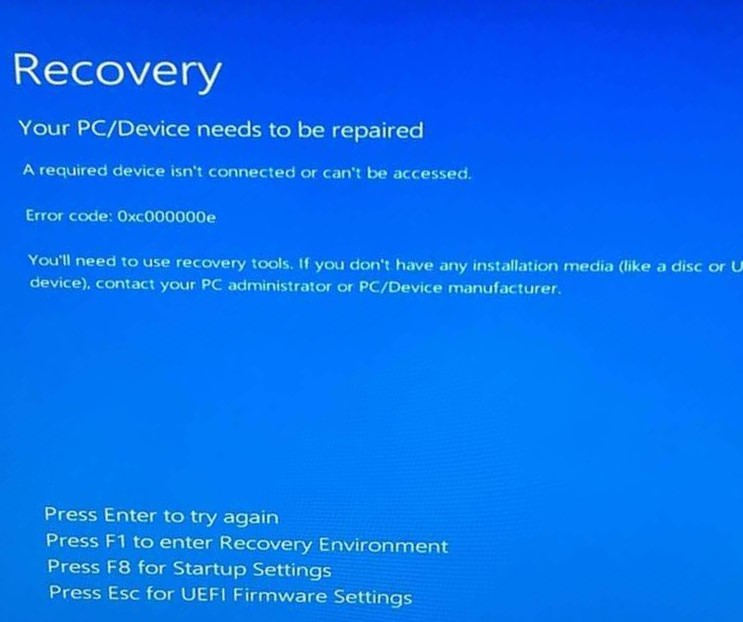
\includegraphics[width=.8\linewidth]{prob2.jpg}
     \caption{"Recovery"}\label{Fig:Data2}
   \end{minipage}
\end{figure}



\subsection{Tool 2: NeuralSAT}
Pentru a aplica benchmark-ul și a primi rezultatele am folosit urmatoarea instrucțiune pe care am rulat-o in folderul "neuralsat-pt201" aflat în "neuralsat": 
\begin{lstlisting}[style=bashstyle]
    python3 neuralsat.py
\end{lstlisting}
Pentru acest tool am folosit un program în limbajul Python personalizat deoarece NeuralSAT acceptă doar instrucțiuni de forma: 
\begin{lstlisting}[style=bashstyle]
    python3 main.py --net "example/onnx/mnistfc-medium-net-554.onnx" --spec "example/vnnlib/test.vnnlib"
\end{lstlisting} \par
Pentru a rula datasetul în environment-ul neuralsat, sunt necesare 2 argumente: "--net" care va fi urmat de fișierul cu extensia ".onnx", și "--spec" urmat de fișierul cu extensia ".vnnlib". Cele 2 argumente sunt cruciale pentru acest environment, iar ca soluție pentru a nu fi nevoie de executarea pe rând a 186 de instrucțiuni, am creat fișierul "neuralsat.py" care are rolul de a automatiza procesul. Acesta execută comenzile pentru fiecare combinație de fișiere, le afișează în terminal și le adaugă într-un fișier pentru a putea fi mai accesibile. Am folosit librăria "tqdm" pentru a afișa progresul parcurs din momentul începerii executiei unei combinații de fișiere până la afișarea rezultatului aferent acesteia (Figura 16). De asemenea, am implementat și un tracker pentru a gestiona numărul de combinații care au fost executate. (Figure 17). \par
\begin{figure}[!htb]
   \begin{minipage}{0.48\textwidth}
     \centering
     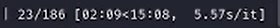
\includegraphics[width=.8\linewidth]{progres1.jpg}
     \caption{Bara de Progress}\label{Fig:Data1}
   \end{minipage}\hfill
   \begin{minipage}{0.48\textwidth}
     \centering
     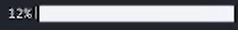
\includegraphics[width=.8\linewidth]{Untitled.jpg}
     \caption{Tracker-ul Execuțiilor}\label{Fig:Data2}
   \end{minipage}
\end{figure}
Ca și rezultate, acestea pot fi vizualizate în fișierul "rezultat\_neuralsat.txt" \cite{ref3}, dar și în tabelul "results\_NeuralSat.csv" \cite{ref4}, unde se pot observa diferențele dintre rezultatele de la competiția din 2023 și rezultatele la care am reușit să ajungem noi. În Figura 18 am evidențiat 3 tipuri de rezultate din fișierul "results\_NeuralSat.csv".  \par
\begin{figure}[h!]
  \centering
    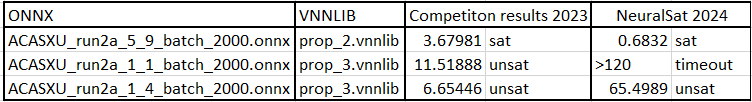
\includegraphics[width=0.9\textwidth]{rezultat2.png}
    \caption{Exemple din fisierul results\_NeuralSat.csv}
\end{figure}
Programul a returnat un total de 46 de cazuri satisfiabile (un-safe), 120 nesatisfiabile (safe), dar și 20 unknown (timeout). Figura 19 reprezintă procentul pe care fiecare tip de rezultat îl reprezintă din totalul de 186 de instanțe. \par
\newpage
\begin{figure}[!htb]
   \begin{minipage}{0.48\textwidth}
     \centering
     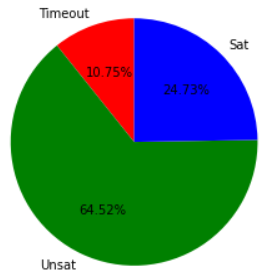
\includegraphics[width=.65\linewidth]{diag3.png}
     \caption{Diagrama Rezultatelor}\label{Fig:Data1}
   \end{minipage}\hfill
   \begin{minipage}{0.48\textwidth}
     \centering
     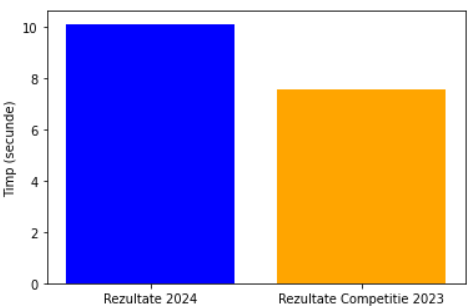
\includegraphics[width=1\linewidth]{diag4.png}
     \caption{Comparare Timp Mediu}\label{Fig:Data2}
   \end{minipage}
\end{figure}
Satisfiabilitatea a fost aceeași ca și în rezultatele din 2023 pentru rezultatele care au fost verificate cu succes (sat, unsat), numai timpul de verificare a fost diferit într-o mare măsură. Timpul de verificare pentru rezultatele satisfiabile a fost considerabil de mic față de cele nesatisfiabile, dar o diferență asemănătoare a fost prezentă și în competiția trecută. De asemenea, timpul mediu de verificare pe care am reușit să-l obținem este cu aproximativ 33.39\% mai mare decât cel obținut în competiția din 2023 (Figura 20), dar de această dată am oprit timeout-ul la 120 de secunde. Programul a afișat 20 de rezultate cu răspunsul "timeout" deoarece nu a reușit să ajungă la un rezultat, iar timpul de verificare a expirat. Am încercat reverificarea pe rând a fișierelor cu rezultat "unknown", dar după numeroase minute de așteptare, programul a returnat rezultatul "killed" (Figure 21). \par
\begin{figure}[h!]
  \centering
    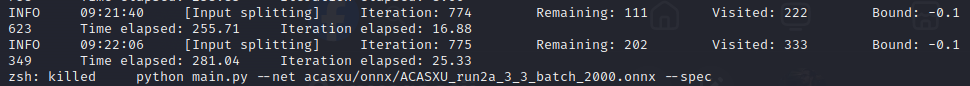
\includegraphics[width=1\textwidth]{killed.png}
    \caption{Eroare "killed"}
\end{figure}
\section{Sumar al Rezultatelor}
Prin furnizarea unui fișier model ONNX și a unui fișier de specificații VNNLIB fiecărui instrument, rezultatul indică dacă există un contraexemplu, adică o situație în care toate condițiile din specificație sunt adevărate dat fiind modelul. Dacă există un contraexemplu, rezultatul este notat cu SAT (Satisfiabil). În caz contrar, este notat cu UNSAT (Nesatisfiabil). În unele situații, totuși, un instrument poate să nu poată să tragă o concluzie pentru verificare și va furniza ca rezultat UNKNOWN. În plus, deoarece instrumentele sunt concepute pentru aceste competiții în care scorurile depind și de timpul de execuție, dacă un instrument nu poate finaliza verificarea într-un interval de timp specificat, algoritmul este întrerupt și va fi furnizat rezultatul TIMEOUT.\par
În cazul experimentului pe care l-am efectuat, au existat 47 de contraexemple atunci când am aplicat $\alpha$-$\beta$-CROWN asupra datasetului AcasXu și respectiv 46 la aplicarea tool-ului NeuralSat. În competiția de anul trecut, timpul maxim de verificare a fost setat la 116 secunde pentru a nu depăși totalul de 6 ore de rulare, iar pentru cele 2 tool-uri și datasetul pe care le-am ales, au primit doar un rezultat "timeout" pentru NeuralSat. În schimb, în urma rezultatelor la care am reușit să ajungem, am identificat 27 de ieșiri "timeout" pentru $\alpha$-$\beta$-CROWN, respectiv 20 pentru NeuralSAT. Din acest fapt am dedus că instrumentele nu au reușit să tragă o concluzie pentru verificare în timp util. Timpul mediu rezultat în urma execuției celor 2 tool-uri este considerabil de diferit de la un tool la altul. Acest lucru este datorat faptului că pentru $\alpha$-$\beta$-CROWN timpul este compus și din secundele acumulate în urma rezultatelor 'unknown', pe când la NeuralSat acest tip de rezultate aveau un timp ne­definit, ajungându-se la eroarea 'killed' despre care am discutat mai sus. Pentru a evita stricarea programului, am setat limita de secunde la 120 și am adăugat în fișierul 'neuralsat.py' comenzi pentru a trece la următoarea combinație dacă timpul de verificare a depășit limita impusă de noi.\par
Tabelul "Table 1" conține rezumatul rezultatelor în urma rulării celor 2 tool-uri asupra dataset-ului AcasXu.\par
    \begin{table}[h]
    \centering
    \begin{tabular}{cccccc}
        \toprule
        \textbf{Tool} & \textbf{Total} & \textbf{SAT} & \textbf{UNSAT} & \textbf{Timeout} & \textbf{Timpul mediu}\\ 
        \midrule
        $\alpha$-$\beta$-CROWN & 186 & 47 & 112 & 27 & 88.362\\
        neuralSAT & 186 & 46 & 120 & 20 & 10.10\\
        \bottomrule
    \end{tabular}
    \caption{Rezultate}
    \label{tab:a}
\end{table}
Pentru a calcula scorul am folosit următoarele punctaje extrase din regulile competiției:
\begin{itemize}
  \item \textbf{Rezultat Nesatisfiabil:} 10 puncte;
  \item \textbf{Rezultat Satifiabil:} 10 puncte;
  \item \textbf{Rezultat Incorect:} -150 puncte.
\end{itemize}
În Tabelul 2 putem identifica următoarele: Verified (Unsat), Falsified (Sat), Fastest, Penalty (Numărul de diferențe față de competiția trecută), Score (Punctajul obținut din adunarea tuturor rezultatelor sat \& unsat înmulțite cu 10. Din rezultat se scade numărul penalităților înmulțit cu 150) și Percent (Cât la sută din maximul de 1860 de puncte s-a obținut).
    \begin{table}[h]
    \centering
    \begin{tabular}{cccccccc}
        \toprule
        \textbf{\#} &\textbf{Tool} & \textbf{Verified} & \textbf{Falsified} & \textbf{Fastest} & \textbf{Penalty} & \textbf{Score} & \textbf{Percent}\\ 
        \midrule
        1 & $\alpha$-$\beta$-CROWN & 112 & 47 & 0 & 27 & -2460 & 0\%\\
        2 & neuralSAT & 120 & 46 & 0 & 19 & -1190 & 0\%\\
        \bottomrule
    \end{tabular}
    \caption{Benchmark 2024-acasxu}
    \label{tab:a}
\end{table}
\section{Concluzii}
În concluzie, scopul acestui proiect a fost atins deoarece am reușit instalarea și antrenarea celor două tool-uri ($\alpha$-$\beta$-CROWN \& neuralSat) asupra datasetului AcasXU. Rezultatele nu au fost conform așteptărilor deoarece au existat numeroase penalități care au dus la un scor negativ.


\newpage
\bibliography{name}
\bibliographystyle{IEEEtran}
\addcontentsline{toc}{chapter}{Bibliography}


\end{document} 


